% !Mode:: "TeX:UTF-8"	% read in as utf8 file.

\section{Linear Strain Triangle}

\subsection{Nodal displacements}
Each node of Linear Strain Triangular has two degrees of freedom: displacements in the $ x $ and $ y $ directions.

Let $ u_i $ and $ v_i $ represent the node $ i $ displacement components in the $ x $ and $ y $ directions, respectively.

\begin{figure}[h!]
\centering
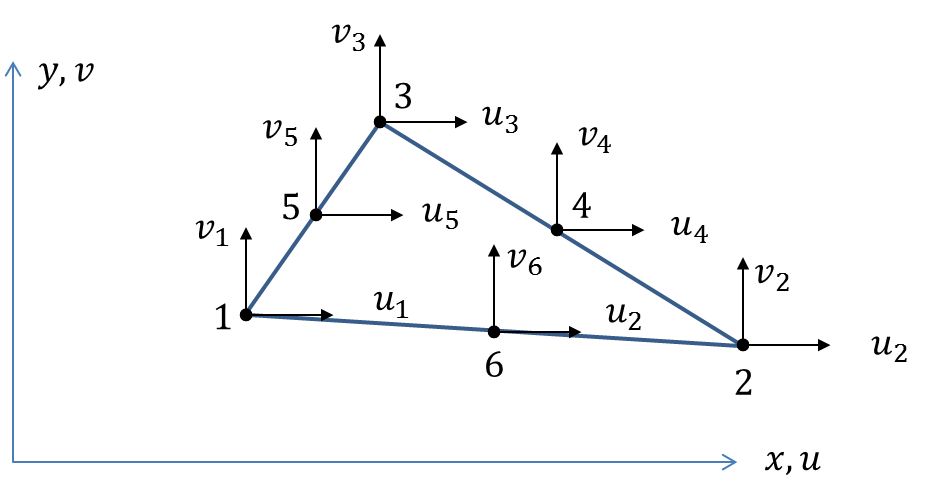
\includegraphics[width=0.7\linewidth]{figures/LST_element}
\caption{Linear strain triangle element}
\label{fig:LST_element}
\end{figure}

\begin{equation}
\mathbf{q}^e = \left\lbrace \begin{array}{c}
q_1 \\ 
q_2 \\ 
q_3 \\ 
q_4 \\ 
q_5 \\ 
q_6 \\
q_7 \\
q_8 \\
q_9 \\
q_{10} \\
q_{11} \\
q_{12}
\end{array} \right\rbrace = \left\lbrace \begin{array}{c}
u_1 \\ 
v_1 \\ 
u_2 \\ 
v_2 \\ 
u_3 \\ 
v_3 \\
u_4 \\
v_4 \\
u_5 \\
v_{5} \\
u_{6} \\
v_{6}
\end{array} \right\rbrace
\end{equation}

\subsection{Shape functions}
The variation of the displacements over the element may be expressed as:

\begin{equation}
\begin{split}
u(x,y) &= a_1 + a_2 x + a_3 y + a_4 x^2 + a_5 x y + a_6 y^2 \\
v(x,y) &= a_7 + a_8 x + a_9 y + a_{10} x^2 + a_{11} x y + a_{12} y^2
\end{split}
\end{equation}

The coefficients $ a_1 $ through $ a_6 $ can be calculated by evaluating the displacement $ u $ at each node.

\begin{equation} \setcounter{MaxMatrixCols}{12}
\boldsymbol{\delta} = \left\lbrace \begin{array}{c}
u(x,y) \\ 
v(x,y)
\end{array} \right \rbrace  = \begin{bmatrix}
1 & x & y & x^2 & xy & y^2 & 0 & 0 & 0 & 0 & 0 & 0 \\ 
0 & 0 & 0 & 0 & 0 & 0 & 1 & x & y & x^2 & xy & y^2
\end{bmatrix} \left\lbrace \begin{array}{c}
a_1 \\ 
a_2 \\ 
a_3 \\ 
a_4 \\ 
a_5 \\ 
a_6
\end{array} \right \rbrace = \mathbf{H}_\delta \mathbf{a}
\end{equation}

To obtain the values for the $ \mathbf{a} $'s substitute the coordinates of the nodal points into the above equations:

\begin{equation}
\left\lbrace \begin{array}{c}
u_1 \\
u_2 \\
\vdots \\
u_6 \\
v_1 \\
\vdots \\
v_5 \\
v_6 \end{array} \right\rbrace = \begin{bmatrix}
1 & x_1 & y_1 & x_1^2 & x_1 y_1 & y_1^2 & 0 & 0 & 0 & 0 & 0 & 0 \\ 
1 & x_2 & y_2 & x_2^2 & x_2 y_2 & y_2^2 & 0 & 0 & 0 & 0 & 0 & 0 \\ 
\vdots & \vdots & \vdots & \vdots & \vdots & \vdots & \vdots & \vdots & \vdots & \vdots & \vdots & \vdots \\ 
1 & x_6 & y_6 & x_6^2 & x_6 y_6 & y_6^2 & 0 & 0 & 0 & 0 & 0 & 0 \\ 
0 & 0 & 0 & 0 & 0 & 0 & 1 & x_1 & y_1 & x_1^2 & x_1 y_1 & y_1^2 \\ 
\vdots & \vdots & \vdots & \vdots & \vdots & \vdots & \vdots & \vdots & \vdots & \vdots & \vdots & \vdots \\ 
0 & 0 & 0 & 0 & 0 & 0 & 1 & x_5 & y_5 & x_5^2 & x_5 y_5 & y_5^2 \\ 
0 & 0 & 0 & 0 & 0 & 0 & 1 & x_6 & y_6 & x_6^2 & x_6 y_6 & y_6^2
\end{bmatrix} \left\lbrace \begin{array}{c}
a_1 \\
a_2 \\
\vdots \\
a_6 \\
a_7 \\
\vdots \\
a_{11} \\
a_{12}
\end{array} \right\rbrace = \mathbf{A}_\delta \mathbf{a}
\end{equation}

Solving for the $ \mathbf{a} $'s:

\begin{equation}
\left\lbrace \begin{array}{c}
a_1 \\
a_2 \\
\vdots \\
a_6 \\
a_7 \\
\vdots \\
a_{11} \\
a_{12}
\end{array} \right\rbrace = \begin{bmatrix}
1 & x_1 & y_1 & x_1^2 & x_1 y_1 & y_1^2 & 0 & 0 & 0 & 0 & 0 & 0 \\ 
1 & x_2 & y_2 & x_2^2 & x_2 y_2 & y_2^2 & 0 & 0 & 0 & 0 & 0 & 0 \\ 
\vdots & \vdots & \vdots & \vdots & \vdots & \vdots & \vdots & \vdots & \vdots & \vdots & \vdots & \vdots \\ 
1 & x_6 & y_6 & x_6^2 & x_6 y_6 & y_6^2 & 0 & 0 & 0 & 0 & 0 & 0 \\ 
0 & 0 & 0 & 0 & 0 & 0 & 1 & x_1 & y_1 & x_1^2 & x_1 y_1 & y_1^2 \\ 
\vdots & \vdots & \vdots & \vdots & \vdots & \vdots & \vdots & \vdots & \vdots & \vdots & \vdots & \vdots \\ 
0 & 0 & 0 & 0 & 0 & 0 & 1 & x_5 & y_5 & x_5^2 & x_5 y_5 & y_5^2 \\ 
0 & 0 & 0 & 0 & 0 & 0 & 1 & x_6 & y_6 & x_6^2 & x_6 y_6 & y_6^2
\end{bmatrix} ^ {-1} \left\lbrace \begin{array}{c}
u_1 \\
u_2 \\
\vdots \\
u_6 \\
v_1 \\
\vdots \\
v_5 \\
v_6 \end{array} \right\rbrace = \mathbf{A}_\delta^{-1} \begin{bmatrix}
\mathbf{u} \\
\mathbf{v}
\end{bmatrix}
\end{equation}

The general displacement expressions in terms of interpolation functions and the nodal degrees of freedom are:

\begin{equation}
\{\delta \} = [N] \{ u \},~~\mathrm{where}~~\mathbf{N} = \mathbf{H}_\delta \mathbf{A}_\delta^{-1}
\end{equation}

\subsection{Element strains}
The strains over two dimensional element are:

\begin{equation}
\left\lbrace \varepsilon \right\rbrace = \left\lbrace \begin{array}{c}
\varepsilon_x \\
\varepsilon_y \\
\varepsilon_{xy}
\end{array} \right\rbrace = \left\lbrace \begin{array}{c}
\frac{\partial u}{\partial x} \\
\frac{\partial v}{\partial y} \\
\frac{\partial u}{\partial y} + \frac{\partial v}{\partial x} \end{array} \right\rbrace
= \begin{bmatrix}
0 & 1 & 0 & 2x & y & 0 & 0 & 0 & 0 & 0 & 0 & 0 \\
0 & 0 & 0 & 0 & 0 & 0 & 0 & 1 & 0 & 0 & x & 2y \\
0 & 0 & 1 & 0 & x & 2y & 0 & 1 & 0 & 2x & y & 0
\end{bmatrix} \left\lbrace \begin{array}{c} 
a_1 \\
a_2 \\
\vdots \\
a_{11} \\
a_{12}
\end{array} \right\rbrace
\end{equation}

Therefore, we have 

\begin{equation}
\left\lbrace \varepsilon \right \rbrace = [B] \left\lbrace q \right\rbrace = \begin{bmatrix}
0 & 1 & 0 & 2x & y & 0 & 0 & 0 & 0 & 0 & 0 & 0 \\
0 & 0 & 0 & 0 & 0 & 0 & 0 & 1 & 0 & 0 & x & 2y \\
0 & 0 & 1 & 0 & x & 2y & 0 & 1 & 0 & 2x & y & 0
\end{bmatrix} \mathbf{A}_\delta^{-1} \left\lbrace \begin{array}{c}
u_1 \\
u_2 \\
\vdots \\
u_6 \\
v_1 \\
\vdots \\
v_5 \\
v_6 \end{array} \right\rbrace
\end{equation}

\subsection{Elemental stresses}
The stresses are given as: 

\begin{equation}
\left\lbrace \begin{array}{c}
\sigma_x \\
\sigma_y \\
\tau_{xy}
\end{array} \right\rbrace = [D] \left\lbrace \begin{array}{c}
\varepsilon_x \\
\varepsilon_y \\
\varepsilon_{xy}
\end{array} \right\rbrace
\end{equation}

For plane stress, $ [D] $ is:

\begin{equation}
[D] = \frac{E}{1-\nu^2} \begin{bmatrix}
1 & \nu & 0 \\
\nu & 1 & 0 \\
0 & 0 & \frac{1-\nu}{2}
\end{bmatrix}
\end{equation}

For plane strain, $ [D] $ is:

\begin{equation}
[D] = \frac{E}{(1+\nu)(1-2\nu)} \begin{bmatrix}
1-\nu & \nu & 0 \\
\nu & 1-\nu & 0 \\
0 & 0 & \frac{1-2\nu}{2}
\end{bmatrix}
\end{equation}

\subsection{Element stiffness matrix}
The stiffness matrix can be defined as:

\begin{equation}
[k] = \int_V [B]^T [D] [B] dV
\end{equation}